\documentclass{standalone}
\usepackage{tikz}
\usetikzlibrary{automata,positioning}

\begin{document}
  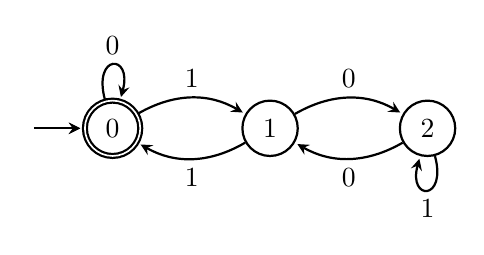
\begin{tikzpicture}[%
    >=stealth,
    shorten >=1pt,
    node distance=2cm,
    on grid,
    auto,
    state/.append style={minimum size=2em},
    thick
  ]
    \node[state, initial, initial text = {}, accepting] (A) {$0$};
    \node[state] (B) [right of=A] {$1$};
    \node[state] (C) [right of=B] {$2$};

    \path[->] (A) +(-1,0) edge (A)
              (A)         edge [loop above] node {$0$} (A)
              (A)         edge [bend left] node {$1$} (B)
              (B)         edge [bend left] node {$0$} (C)
              (B)         edge [bend left] node {$1$} (A)
              (C)         edge [bend left] node {$0$} (B)
              (C)         edge [loop below] node {$1$} (C) ;
  \end{tikzpicture}
\end{document}